\documentclass[aps,superscriptaddress, notitlepage,longbibliography]{revtex4-1}

\usepackage{amsmath}
\usepackage{physics}
\usepackage[pdftex]{graphicx}
\usepackage{xcolor}
\usepackage{hyperref}
\setlength {\marginparwidth }{2cm}
\hypersetup{
    colorlinks,
    citecolor=blue,
    filecolor=black,
    linkcolor=red,
    urlcolor=blue
}

\newcommand{\comment}[1]{{\color{blue}#1}}
\newcommand{\edit}[1]{{\color{purple}#1}}
\newcommand{\del}[1]{{\color{red}\st{#1}}}
\newcommand{\beginsupplement}{%
        \setcounter{table}{0}
        \renewcommand{\thetable}{S\arabic{table}}%
        \setcounter{figure}{0}
        \renewcommand{\thefigure}{S\arabic{figure}}%
     }

\begin{document}

\title{Single-cell Type Order Parameters (scTOP): A parameterless, non-stochastic algorithm for tracking cell identity using single-cell atlases}

\author{Maria Yampolskaya}
\email{mariay@bu.edu}
\affiliation{Department of Physics, Boston University, Boston, MA 02215, USA}

\author{Pankaj Mehta}
\email{pankajm@bu.edu}
\affiliation{Department of Physics, Boston University, Boston, MA 02215, USA}
\affiliation{Faculty of Computing and Data Science, Boston University, Boston, MA 02215, USA}
\affiliation{Biological Design Center, Boston University, Boston, MA 02215, USA}


\begin{abstract}
To better understand cell-level phenotypic development and reprogramming, scientists are generating an abundance of single-cell RNA-sequencing (scRNA-seq) tissue atlases, lineage tracing studies, and other measurements. Using this high-dimensional, noisy data to identify cell type and understand the dynamics of cell fate transitions remains an ongoing problem. We introduce single-cell Type Order Parameters (scTOP), an epigenetic-landscape-inspired algorithm to locate individual cells in the coordinate space of known cell types. We use existing human and mouse datasets that span across the body to show scTOP reliably identifies cell type and traces the developmental progress of cells. scTOP visualizes the trajectory of lineage tracing experiments by directly comparing each timepoint state to the final fates. By tracking cells in cell type space, scTOP provides the technical foundation to understand in vivo developmental paths and possible bifurcations in the phenotypic landscape.
\end{abstract}

\maketitle

\section{Introduction}
Many adult animals exhibit hundreds of specialized cell states, all of which arose from a small number of embryonic cells. In early stages of development, embryonic cells possess the transcriptomic flexibility to become virtually any of the eventual cell fates. The questions of how and why cells end up in one fate or another is of interest both in biology and the physics of self-organizing systems. Understanding which cell fate transitions are possible is necessary to establish a theoretical framework for development. Understanding transitions is also important for developing directed differentiation protocols to engineer cells in vitro.

An indispensable way to probe cell type is by measuring the transcriptome. Capturing and quantifying the amounts of mRNA in a cell provides a snapshot of its phenotype. With the advancement of single-cell RNA-sequencing (scRNA-seq), gene expression data of individual cells are being produced at unprecedented rates. Typical scRNA-seq measurements involve thousands of genes and dozens to millions of cells, resulting in high-dimensional data. Due to the technical challenges of sequencing RNA, the resulting data is noisy and sparse \cite{lahnemann_eleven_2020}. Genes with relatively low expression are often recorded as not being expressed at all, resulting in zero-counts called “dropouts”. Experimental-to-experiment differences in sequencing method, platform, and other difficult-to-standardize conditions result in technical variations in scRNA-seq measurements called “batch effects.” These challenges merit careful consideration of how to normalize and analyze the data in a way that permits study of biological variation without obfuscation by technical variation.

clustering, trajectory inference, and automatic cell identification are three major computational approaches to examining cell fate using scRNA-seq data. Clustering involves applying dimensional reduction (such as UMAP \cite{mcinnes_umap_2018} or SPRING \cite{weinreb_spring_2018}) to visualize the data in two dimensions, then using unsupervised clustering to group individual cells. These groups are often manually annotated according to expression levels of marker genes. Trajectory inference analysis arranges cells on a manifold and assigns pseudo-times according to transcriptomic similarity. There are also methods like partition-based graph abstraction \cite{wolf_paga_2019} that purport to combine clustering and trajectory inference to simultaneously calculate pseudo-times and provide discrete labels at varying resolutions. Machine learning classifiers such as support vector machines are able to automatically identify cells with high accuracy \cite{abdelaal_comparison_2019}.

Although there are many useful computational tools to extract cell identity from scRNA-seq, the common methods share certain limitations. Dimensional reduction is often one of the first steps to analyze scRNA-seq data, but current methods highly distort cell-to-cell and cluster-to-cluster quantitative relationships \cite{chari_specious_2021}. Distorted embeddings inconsistently represent distances between individual data points and between cell types, which makes it difficult to interpret cell fate transitions. This issue carries over to trajectory inference, since it uses nearest neighbors which can vary substantially according to the embedding. Another limitation is the lack of reproducibility inherent in stochastic machine learning methods \cite{wattenberg_how_2016} like t-SNE and UMAP, which output different results whenever they are executed. Depending on exactly which data points are included, the output distribution may change significantly, even of data points that are retained from one iteration to another. The algorithm results also widely vary depending on input parameters such as perplexity. These parameters insert implicit assumptions about the locality of the data features. Since different papers use different parameters, each use of these algorithms applies different assumptions, rendering quantitative comparison between outputs impossible.

Ideally, an algorithm to explore cell fate transitions using scRNA-seq data would overcome these limitations by having explicit assumptions that can be kept consistent between analyses. Reproducibility would be further enhanced by a deterministic program. Currently, the axes of dimensional reduction outputs are difficult to interpret since they represent a complicated calculation of high-dimensional distance. Analysis would be improved if output axes were intuitive and remained meaningful from one algorithm iteration to another. This would require distances between points and clusters to remain undistorted after application. Meaningful axes could quantify cell type instead of assigning discrete identity labels, enabling numerical examination of transitions.

Our algorithm, single-cell Type Order Parameters (scTOP), reproducibly projects scRNA-seq data onto the dimensions of known cell types. Order parameters are variables whose values change as the system’s phase changes. Inspired by the epigenetic landscape and spin glass physics, scTOP treats cell types as phases and calculates the order parameters for transitions between them. It builds on previous work applying attractor-based order parameters to bulk RNA-sequencing\cite{lang_epigenetic_2014} \cite{dame_thyroid_2017}\cite{pusuluri_cellular_2017} \cite{ikonomou_vivo_2020}. The inputs into scTOP are the scRNA-seq measurements of query data as well as a reference basis of known cell types. The reference basis contains the archetypal gene expression profiles for the known cell types. scTOP outputs the coordinates of the query data in cell type space; each output dimension corresponds to a measure of similarity between the query data and one of the known cell types in the reference basis. Instead of reducing the data to two arbitrary dimensions, scTOP reduces the data to the number of provided cell types. With scTOP, it’s possible to visualize the path of a cell on axes measuring similarity to the most relevant cell types. The assumptions of the algorithm are explicit: that the known cell types are dynamical system attractors, and that the provided reference basis accurately represents the gene expression profiles of the known cell types. scTOP allows direct comparison between datasets, since the coordinates of and distances between data points do not change from application to application unless the reference basis is changed. scTOP is a robust, deterministic algorithm that creates consistent, intuitive axes on which to observe cell fate transitions.

In this paper, we show that scTOP reliably quantifies cell identity. It classifies cell type of individual cells with high accuracy, as demonstrated using mouse and human samples from lungs, brains, and organs throughout the body. By analyzing lineage tracing data and embryonic development data, we also establish scTOP’s capacity to quantify transitions between cell types. 

We present scTOP in the easy-to-use forms of a Python package, available on the Python Package Index [link] and Github [link], and an R package, available on Bioconductor [link] and Github [link].

\section{Methods}
\begin{figure}
	\centering
		\includegraphics[scale=0.8]{figs/fig1.pdf}
	\caption{Steps involved in the scTOP algorithm. (a) Each sample in the query data is pre-processed independently of the other samples in the dataset. “Sample” may refer to either an individual cell sample or the average of cell samples corresponding to a tissue or population of interest. The former leads to individual cell analysis, and step 0 would be a matrix of single-cell RNA counts. The latter, which we call aggregate scoring, leads to tissue- or population- level analysis, and step 0 would involve a matrix where each “sample” column corresponds to an average of single-cell RNA counts. (b) Single-cell RNA-seq atlases, such as the Mouse Cell Atlas, are used to define the reference basis in the algorithm. (c) scTOP scores are the projections of query data onto the non-orthogonal subspace of cell types. Since there is no statistical fitting, no tuning parameters are involved. (d, e) show the process of finding scTOP scores, and the illustrated cell-type space has as many dimensions as there are cell types in the reference basis. We can visualize this concept in 1, 2, or 3 dimensions, depending on which cell types are most relevant. In the 3-dimensional case, the shadows on the bounds of the scatter plot are included to better illustrate the position of points in 3-dimensional space. (d) The process of finding scTOP scores for aggregate samples, which are averaged RNA counts for a population of interest. Note that the aggregate score tends to be higher than the average score of the individual cells (see 1e), since averaging over the RNA counts *before* scoring reduces the impact of noise. (e) The process of finding scTOP scores for individual cell samples.}
	\label{FIG:1}
\end{figure}

To calculate cell type similarity scores, scTOP uses a linear algebra projection method inspired by the concept of cell types as attractors in a dynamical system \cite{huang_cell_2005}. This projection method has been applied previously to bulk RNA-seq samples, and we will summarize the theoretical background here \cite{lang_epigenetic_2014}. A cell type is a state of the gene regulatory network, so a natural way to represent attractors in this system is with an attractor neural network. If we represent each gene as a node in a network with an associated value measuring gene expression (positive value representing high gene expression, low value indicating low gene expression), then a cell type may be denoted by a vector of gene expression values. Cell types are often highly similar in their patterns of gene regulation. Kanter and Sompolinsky \cite{kanter_associative_1987} defined a pattern storage method for spin-glass-like neural networks where even correlated patterns robustly act as attractors. For the same system, they also defined order parameters $a^{\mu}$ which are de-correlated versions of the conventional spin glass order parameter, magnetization. $a^{\mu}$ measures the similarity between a given network state and the network state $\mu$, which is a stored pattern (in our case, a gene regulatory pattern that corresponds to a cell type). As Lang et al. have shown, the order parameters $a^{\mu}$ provided an excellent similarity score for analyzing bulk RNA-seq data. However, the cells digested by bulk RNA-seq may be in different stages of differentiation, and bulk processing renders it impossible to measure cell fate transitions beyond an average tissue state. scTOP uses the same order parameters, $a^{\mu}$, to track cell type at the resolution of individual cells, making it possible to directly observe cells in different stages of differentiation.

In pre-processing, the raw RNA-seq count data are first normalized, then z-scored. The details of the process and its effects on data distributions are described in Appendix section \ref{preprocessing}.

The structure of pre-processing before applying the projection method is a vital component of the algorithm, as shown in figure \ref{FIG:1} (a). Each sample is pre-processed independently, unlike other algorithms which process data across samples to find, for example, the most variable genes. Depending on the particular application of scTOP, "sample" may refer to either an individual cell or the average expression levels of a subpopulation of cells. By processing each sample independently, the output for one sample is independent of which samples are analyzed alongside that one sample. scTOP involves one-shot learning, and there is no stochasticity involved; the algorithm will produce the same output regardless of the particular instance of execution. There are no hyper-parameters involved in the training, which bypasses another source of bias. The only assumptions involved in the algorithm are explicit: that the gene expression profiles included in the reference basis are truly representative of the relevant cell types, and that the cell types included are indeed distinct cell phenotypes.

Constructing a representative, accurate reference basis that is relevant to the data being analyzed is vital to the scTOP algorithm. This process is shown in figure \ref{FIG:1} (b). First, relevant single-cell RNA-seq atlases are gathered to be processed. For example, in analyzing mouse lung cells, we used the Mouse Cell Atlas \cite{noauthor_mapping_nodate}, which contains single-cell samples of mouse tissues across all major organs. Once the relevant atlases are identified, we take an average across each cell population that corresponds to a distinct cell type. It is important that enough cells are included in each average, in order to mitigate the potent effects of noise. The minimum sample size to achieve reasonable results is 200 cells. Noise affects the algorithm most strongly when it appears in the basis, since the de-correlation operation involved in the projection separates cells according to the canonical expression levels included in the reference basis. After each cell population is averaged to create the gene expression profiles for the desired cell types, each cell type profile is pre-processed separately. This creates a modular reference basis where cell types can easily be replaced, removed, or added at will. 

Although they were originally inspired by attractor neural networks and spin glass physics, the order parameters $a^{\mu}$ can also be understood as non-orthogonal projections onto the subspace of cell type space. This idea is shown in figure \ref{FIG:1} (c). A single-cell RNA-seq measurement of a sample produces a list of values corresponding to the expression levels of different genes, and thus can be conceptualized as a vector in $G$-dimensional gene expression space, where $G$ is the number of genes. Single-cell RNA-seq atlases provide reference gene expression profiles for hundreds of known cell types; these reference profiles also exist as vectors in gene expression space. If we compile a reference basis consisting of reference profiles corresponding to cell types, these vectors span a $C$-dimensional subspace of gene expression space, where $C$ is the number of cell types in the basis. There are far more genes than cell types: $C < G$. We can project the measured sample vector onto the cell type subspace in order to find the coordinates in cell type space, which enables identification of individual cells and tissues. Since the cell type profiles are largely correlated, they form a non-orthogonal subspace, and the projection onto this space is a non-orthogonal projection.

We can write the sample vector as a sum of the projected components and the component perpendicular to the cell type subspace: $S_i = \sum_\mu a^{\mu} \xi^{\mu}_i + S^{\perp}_i$. $S_i$ is the expression level of the $i$th gene in the measured sample. $a^{\mu}$ is the projection of the sample vector onto cell type $\mu$. $\xi^{\mu}_i$ is the expression level of the $i$th gene in the reference profile of cell type $\mu$. $S^{\perp}_i$ is the expression level of the $i$th gene of the component of the sample vector that is perpendicular to the cell type subspace. $S^{\perp}$ is the part of the sample vector that is not explained by the known cell types. It results from biological processes such as cell cycle variation and non-biological sources such as scRNA-seq noise. 

There are two types of scTOP scores: aggregate and individual. The aggregate scoring method is useful for analyzing identified sub-populations of data at once. The scores tend to be higher, since aggregating gene expression data decreases the effects of noise. In aggregate scoring, the raw RNA count data is averaged across each sub-population, and then these average gene expression profiles are pre-processed and projected onto the reference basis. See figure \ref{FIG:1} (d). The resulting scTOP score provides the location of the sub-population in the cell type dimensions specified by the reference basis, which can be visualized in one, two, or three dimensions by selecting one, two, or three relevant cell types. In individual scoring, as shown in figure \ref{FIG:1} (e), each individual cell is pre-processed and projected onto the reference basis separately. Due to the well-documented effects of scRNA-seq noise, the resulting scores tend to be lower. Nonetheless, the resulting scores are able to accurately and reproducibly identify and track individual cells through cell type space, in whatever number of dimensions (i.e. cell types) one chooses.

The crux of scTOP is choosing a good reference basis. scTOP scores are reliable when the input reference basis incorporates many cells and represents a wide, relevant set of specialized cell types. Since scRNA-seq data is noisy and dropout is prevalent, many cells of each reference cell type must be included in order to create representative gene expression profiles. The choice of cell types in the basis is vital, too. The main underlying assumption of scTOP is that the reference cell types accurately represent attractors of the gene regulatory network. If the cell types aren’t well-differentiated from one another, as in early embryonic development or certain stromal cells when compared between organs, the resulting scTOP scores may be unreliable; they may change drastically when the basis is only slightly changed, or they may be incoherent. More information on the limitations of scTOP may be found in appendix [insert appendix num.].

The accuracy of cell type information that scTOP can extract from scRNA-seq is limited by the low signal-to-noise ratio. As shown in appendix [insert appendix num.], the scTOP scores for false identities form a Gaussian distribution around zero. These distributions give an estimate of error. In aggregate scTOP scoring, RNA counts are averaged across a population and the resulting score is generally higher for relevant cell types than the average individual scTOP score for the same population. This is because the averaging step in aggregate scoring mitigates the effects of sparsity and noise in the RNA count matrices.

\section{Results}

\subsection{Benchmarking and validation: Classification of cell fate}
scTOP scores reliably and accurately identify the cell types of individual cells as well as of clusters of cells. To show this, we applied the algorithm to several scRNA-seq datasets across species and across laboratories. scTOP is organism-agnostic as long as an appropriate reference basis is used. Mice and humans are among the most common subjects of scRNA-seq measurements. Many atlases across organs and stages of development have been created for both species. We used some of these atlases, such as the Mouse Cell Atlas \cite{noauthor_mapping_nodate} and the Atlas of Lung Development \cite{negretti_single-cell_2021}, as reference bases to analyze datasets from various sources.

Table \ref{table:1} lists each of the datasets examined in this paper with their respective scTOP score accuracies. "TopN" refers to the percent of cells whose true cell types were in the top "N" scTOP scores, with a score greater than 0.1. "Unspecified" refers to the percent of cells for which the highest scTOP score was less than 0.1; this represents a failure of the algorithm to confidently identify the cell. The accuracies across species and tissues are high and the unspecified percentages are very low, even in the dataset exceeding a million cells.

\begin{table}[h!]
\centering
\begin{tabular}{| c | c | c | c | c | c | c |}
\hline
Query Data & Species & Reference Basis & Top1 (percent) & Top3 (percent) & Unspecified (percent) & Total cells \\ 
\hline
Kotton lab & Mouse & Mouse Cell Atlas & 97.19 & 99.77 & 2.69 & 4,805 \\ 
\hline
Brain atlas & Mouse & Self & 86.28 & 96.89 & 1.78 & 1,161,041 \\
\hline
CellBench & Human & Self & 100 & 100 & 0 & 2,822 \\
\hline
Lung atlas & Human & Self & 79.78 & 85.16 & 3.32 & 2,952 \\  
\hline
\hline
Data set & Species & Reference Basis & Top1 (percent) & Top3 (percent) & Unspecified (percent) & Number of cell types \\
\hline
Mouse Cell Atlas & Mouse & Tabula Muris & 79.17 & 87.5 & 0 & 48 \\
\hline

\end{tabular}
\caption{Accuracy scores of included sample types for each the described data sets.}
\label{table:1}
\end{table}

To demonstrate the efficacy of scTOP in the case where the reference basis and query data come from different sources, we projected mouse lung data from Herriges et al. \cite{herriges_durable_2022} onto the mouse cell atlas. The Herriges et al. b dataset  measures gene expression levels of six different specialized lung types from mice used as control samples. See figure \ref{FIG:2} (a). The reference basis used to find the individual scTOP scores for this data set was derived from the Mouse Cell Atlas. Despite the fact that the Kotton lab dataset and the Mouse Cell Atlas were created in different laboratories and different sequencing methods, the resulting scTOP scores distinctly separate the cells from the Kotton laboratory. The resulting clusters agree with the annotations of the true cell type provided by the Kotton laboratory.

The mouse brain atlas\cite{yao_taxonomy_2021} sequenced over one million cells and clustered them into 42 subclasses and 101 supertypes. For a reference basis, we reserved a subset of 200 cells from each of the identified subclasses to use as training data. The test data, from which the accuracy score was calculated, was the remaining cells of each type not included in the training data. Ten different cell types are visualized in a grid in figure \ref{FIG:2} (b). The color of each grid square corresponds to the average scTOP score of cells annotated as the type on the y-axis, with the cell type corresponding to the scTOP dimension on the x-axis. As shown by the distinct blue diagonal, the average scTOP score correctly matches the corresponding annotated cell type.

scTOP correctly identifies individual cells, and it can also identify the tissue to which a population of cells belongs. As shown in \ref{FIG:2} (c), we found the aggregate scTOP scores for cells from the Mouse Cell Atlas projected onto the reference basis of Tabula Muris organs \cite{schaum_single-cell_2018}. Most cell types were correctly and strongly identified with the annotated tissue of origin. Parenchymal cell types were the most associated with the correct organ, while stromal cells were sometimes misidentified -- for example, the mammary gland endothelial cells. This is consistent with the fact that stromal cells are less specified to each organ. A discussion of the accuracy of scTOP when applied to stromal types versus parenchymal types may be found in appendix \ref{failure_cases}.

\begin{figure}
	\centering
		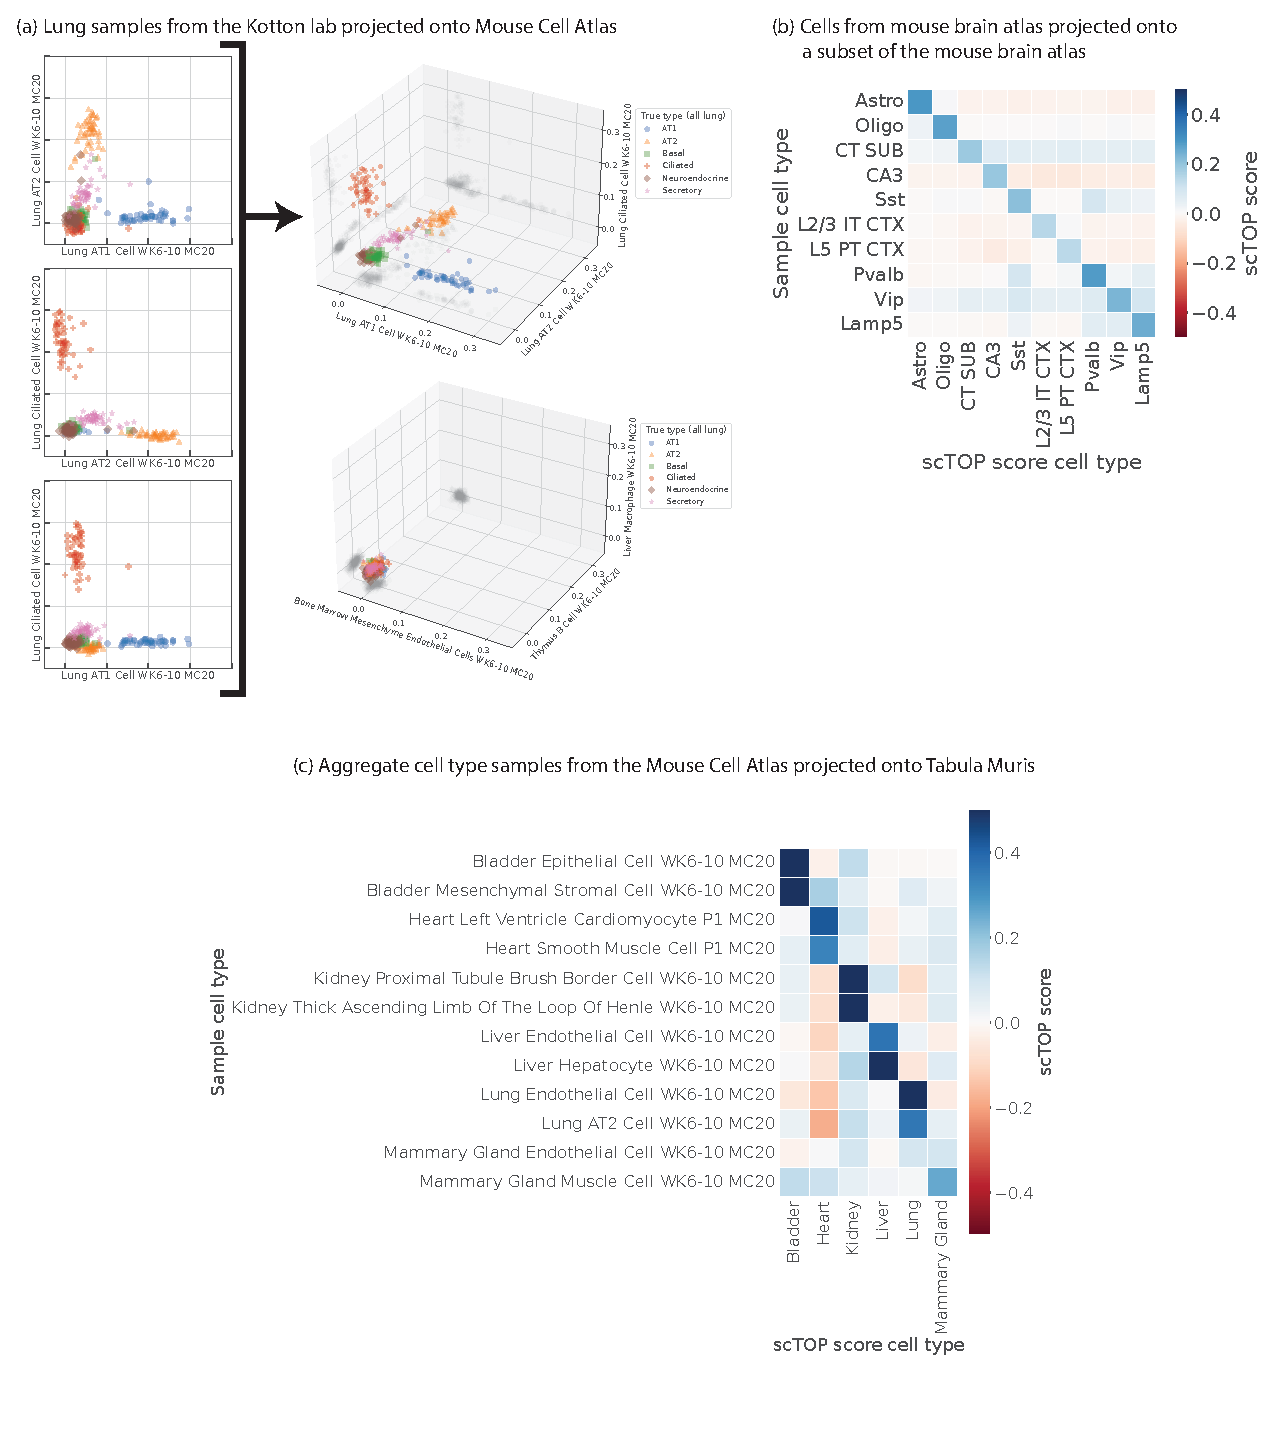
\includegraphics[scale=0.7]{figs/fig2.pdf}
	\caption{scTOP identifies mouse cell types. (a) Using the Mouse Cell Atlas as the reference basis, we show that mouse lung types separate clearly on scTOP score axes. The data points correspond to individual cells, and the marker shape and color indicate the "true type" as determined by annotations from Herriges et al. The axes used are scTOP scores for similarity with lung ciliated cells and alveolar types I and II. We also plotted the scTOP scores for the same data compared to random, irrelevant cell types, showing that the scores are tightly distributed around zero, as expected. (b) A subset of cells from the Mouse Brain Atlas are used as the reference basis to query other cells from the same data set. The shade of each bin corresponds to the average scTOP score for individual cells of the type indicated on the y-axis, compared to the reference types on the x-axis. The diagonal indicates that scTOP accurately matches query cells to the true reference type. (c) Aggregate samples from the Mouse Cell Atlas are compared to a reference basis consisting of organs from Tabula Muris. The scTOP scores are significantly higher when comparing a cell type with the organ of origin. This coarse-grain identification shows scTOP is able to classify tissues at different resolutions.}
	\label{FIG:2}
\end{figure}

The CellBench dataset \cite{tian_benchmarking_2019} was designed specifically to benchmark scRNA-seq analysis methods. We used the subset of data pertaining to five cancer lines. 200 cells from each line were used as training data to create the reference basis, then the rest of the cells were input as query data. As shown in figure \ref{FIG:3} (a) and table \ref{table:1}, scTOP classifies cell line identity of the test data with 100 percent accuracy.

To further prove the power of scTOP in classifying human samples, we analyzed data from the human lung atlas dataset \cite{travaglini_molecular_2020}. This dataset sequenced thousands of human lung cells and identified 58 phenotypic popoulations. For our analysis, we restricted the training and test data to epithelial and stromal types that had at least 200 cells in each type population. The reference basis was created using 80\% of the cells from each population, and the query data consisted of the remaining 20\% of the data. Figure \ref{FIG:3} (b) shows that the scTOP scores were consistently high in cases where the score type matched the true type of the query.

\begin{figure}
	\centering
		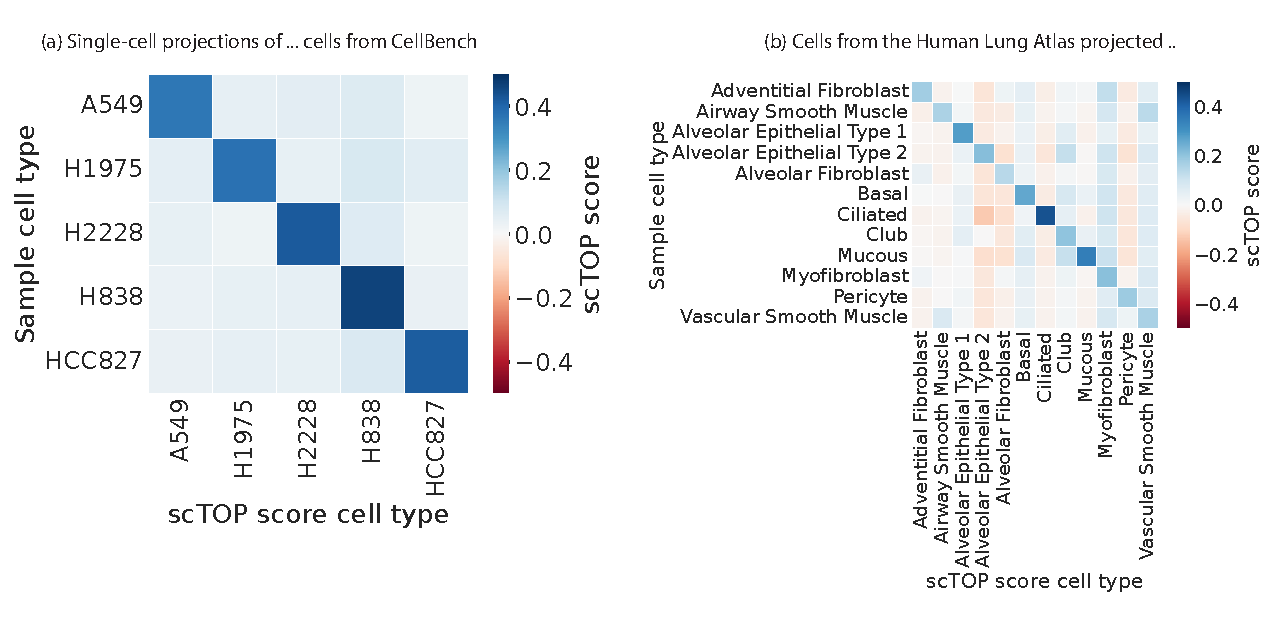
\includegraphics[scale=0.8]{figs/fig3.pdf}
	\caption{scTOP correctly identifies human tissues. (a) The CellBench data set contains human cell cancer lines specifically processed to serve as benchmarking for scRNA-seq algorithms. We take a subset of cells to use as the reference basis in analyzing the rest of the CellBench data. The shade of each bin indicates the average scTOP score for an individual queried cell compared to the cell type indicated on the x-axis. The y-axis lists the true types of the queried cells. The dark diagonal demonstrates the scTOP scores correctly match the queried data to the corresponding true types. (b) Similar to (a), cells from the Human Lung Atlas are compared to a reference basis constructed from cells from the Human Lung Atlas. The colors of the bins correspond to average scTOP scores of individual cells. Again, the diagonal is the most prominent section, showing that cells of the y-axis types are correctly matched to the reference x-axis identities.}
	\label{FIG:3}
\end{figure}

As demonstrated by the diverse data sources examined here, as long as a well-defined reference basis is available, scTOP works well across different measurement conditions, species, organs, and resolutions.

\subsection{Tracking cell type transitions}
The previous section showed that scTOP accurately tracks the developed cell type of individual cells and clusters of cells. Now that we have shown that it correctly identifies the coordinates in cell type space, we can apply it to developing or transitioning cells to see dynamics in cell type space.

The atlas of mouse lung development\cite{negretti_single-cell_2021} contains cells from day 12 embryonic mice to day 14 postnatal mice. They are annotated by cell type, so we can track their differentiation in cell type space using scTOP scores. Figure \ref{FIG:4} (a) shows the aggregate scores of alveolar type I (AT1) and alveolar type II cells (AT2) as the days progress. The x-axis shows the scTOP score for AT1, the y-axis shows AT2, and each point is colored by the scTOP score for early epithelial cell type. The AT1 cells are marked with circles and the AT2 cells are marked with "X"s. It is clear to see that the AT1 cells separate from the AT2 cells early in development, and each one progresses on its separate track. Because scTOP provides us with reference axes that don't change according to whatever data is included, it is possible to track different data points across time on the same axes. Also, these axes give an exact interpretation: they measure the similarity to a canonical known cell type.

The hematopoietic dataset\cite{weinreb_lineage_2020} represents thousands of hematopoietic stem cells and their cloned sister cells in various states of differentiation. scRNA-seq destroys the cell it measures, but by barcoding cloned cells, this dataset traces the lineage of each clone family. Day 2 undifferentiated cells without clones and day 6 differentiated cells without clones were used to form the reference basis. Then, all of the cloned data was analyzed using scTOP. Figure \ref{FIG:4} (c) shows 2D histograms of every single cloned cell regardless of final fate, colored according to the most likely time for each of the bins (see appendix\ref{analysis} for details). The histograms with the day 2 undifferentiated scTOP scores on the x-axis show a clear path to differentiation, starting at high scores for the undifferentiated type at early days (which is represented by the lighter color) then decreasing undifferentiated-type score as time passes, with some portion ending up with high scores for each of the possible differentiated fates.

From the histograms displaying two specialized cell fates, one can see that differentiation pathways for some cell types are mutually suppressive while others form a continuous spectrum between identities. For example, megakaryocytes and monocytes form a distinct L-shape that indicates the development program for each of these types prevents the program of the other; cells are either megakaryocytes, monocytes, or neither, there is no in-between stage. However, the plot for monocytes and neutrophils tells a different story: instead of having a distinct L-shape with narrow distribution along the axes, this plot shows a continuous spectrum of cells that are monocyte-like, neutrophil-like, and every step in-between. 

\begin{figure}
	\centering
		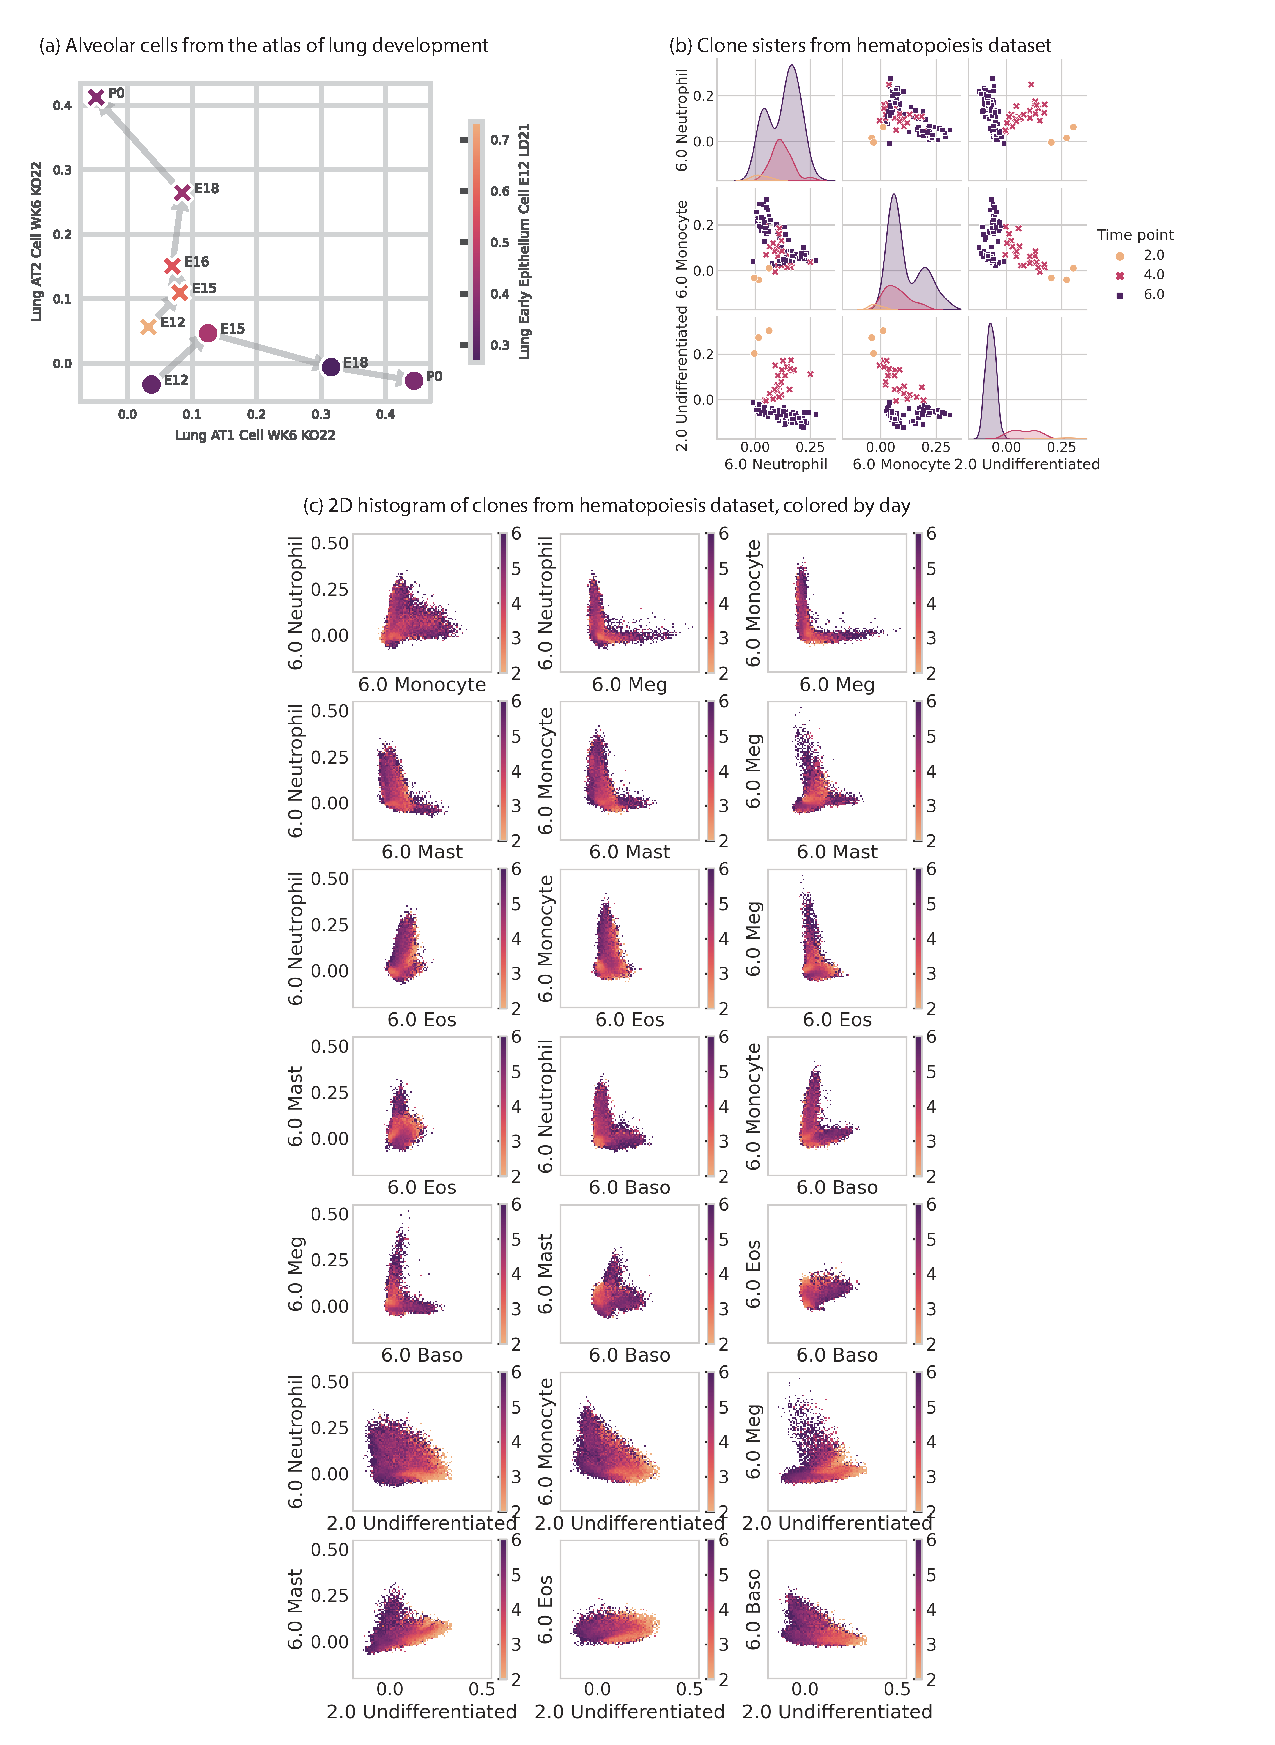
\includegraphics[scale=0.5]{figs/fig4.pdf}
	\caption{Beyond bench-marking: tracing development in cell-type space with scTOP. (a) scTOP illustrates specification of alveolar type I and type II cells in murine embryonic development. Alveolar cells from the Atlas of Lung Development are compared to a reference basis constructed from adult lung cells from Herriges et al. and early epithelial cells from the Atlas of Lung Development. The labels next to each data point indicate the age of the mouse embryo from which lungs were extracted, from post-conception day 12 (E12) to day of birth (P0). The points with O-shaped (X-shaped) markers are alveolar type I (II) cells. The x-axis (y-axis) corresponds to the scTOP score for alveolar type I (II) identities. The shade of each point corresponds to the scTOP score for "early epithelium" identity. (b), (c) scTOP shows cell fate specification of hematopoietic cells using lineage tracing data from Weinreb et al.}
	\label{FIG:4}
\end{figure}


\section{Discussion}

scTOP successfully quantifies cell transitions and enables direct comparison between datasets at the level of individual cells. Using a wide range of data from various sources and species, we have shown that scTOP scores identify cell type in agreement with existing annotations without being limited to discrete cluster labels. scTOP scores provide clear and meaningful axes to observe differentiation, as shown in the cases of epithelial lung development and hematopoietic specification. The input assumptions of our algorithm are explicitly defined by the reference basis, and the results are deterministically determined by linear algebra; scTOP does not require parameter tuning or stochastic machine learning. 

By assigning a continuous value to cell identity, scTOP opens the door to numerical analysis of cell fate decisions. By tracking cell type, it is possible to obtain detailed information on which transitions are possible in vivo. This will provide evidence for mapping out cell lineage trees leading from progenitors to fully-specified fates. By plotting the scTOP scores of differentiating cells, it is possible to see which cell types are mutually repressive and which are close relatives in the lineage tree. Emerging technologies like Live-seq [citation] promise to allow scRNA-seq of live cells without destroying them, and combining this capability with scTOP would allow scientists to track the process of specialization in individual cells without having to settle for lineage tracing of clones.

In addition to revealing in-vivo developmental pathways, scTOP can measure fidelity of engineered cells, as demonstrated in Herriges et al. By locating a cell in cell type space, it is possible to compare the results of directed differentiation protocols and determine which protocol provides the desired result. scTOP can guide reprogramming on a granular level in addition to probing which transitions are possible.

By projecting from gene expression space to cell type space, we can directly track cells in the cell decision landscape. As discussed in Saez et al.\cite{saez_dynamical_nodate}, such an embedding is a crucial step in verifying theoretical models of cell decisions. Many landscape geometries and dynamical systems have been proposed to explain how cell type is decided, but experimental evidence is necessary to test the validity of theoretical models. By providing coordinates in the cell decision landscape, scTOP bridges the gap between theory and experiment.

\section*{Acknowledgments}

Boston University Kilachand Multicellular Design Program NIH NIGMS 1R35GM119461

Simons Investigator in the Mathematical Modeling of Living Systems (MMLS) award to P.M.

\section*{Appendix}
\beginsupplement
\subsection{Pre-processing} \label{preprocessing}

\begin{figure}
	\centering
		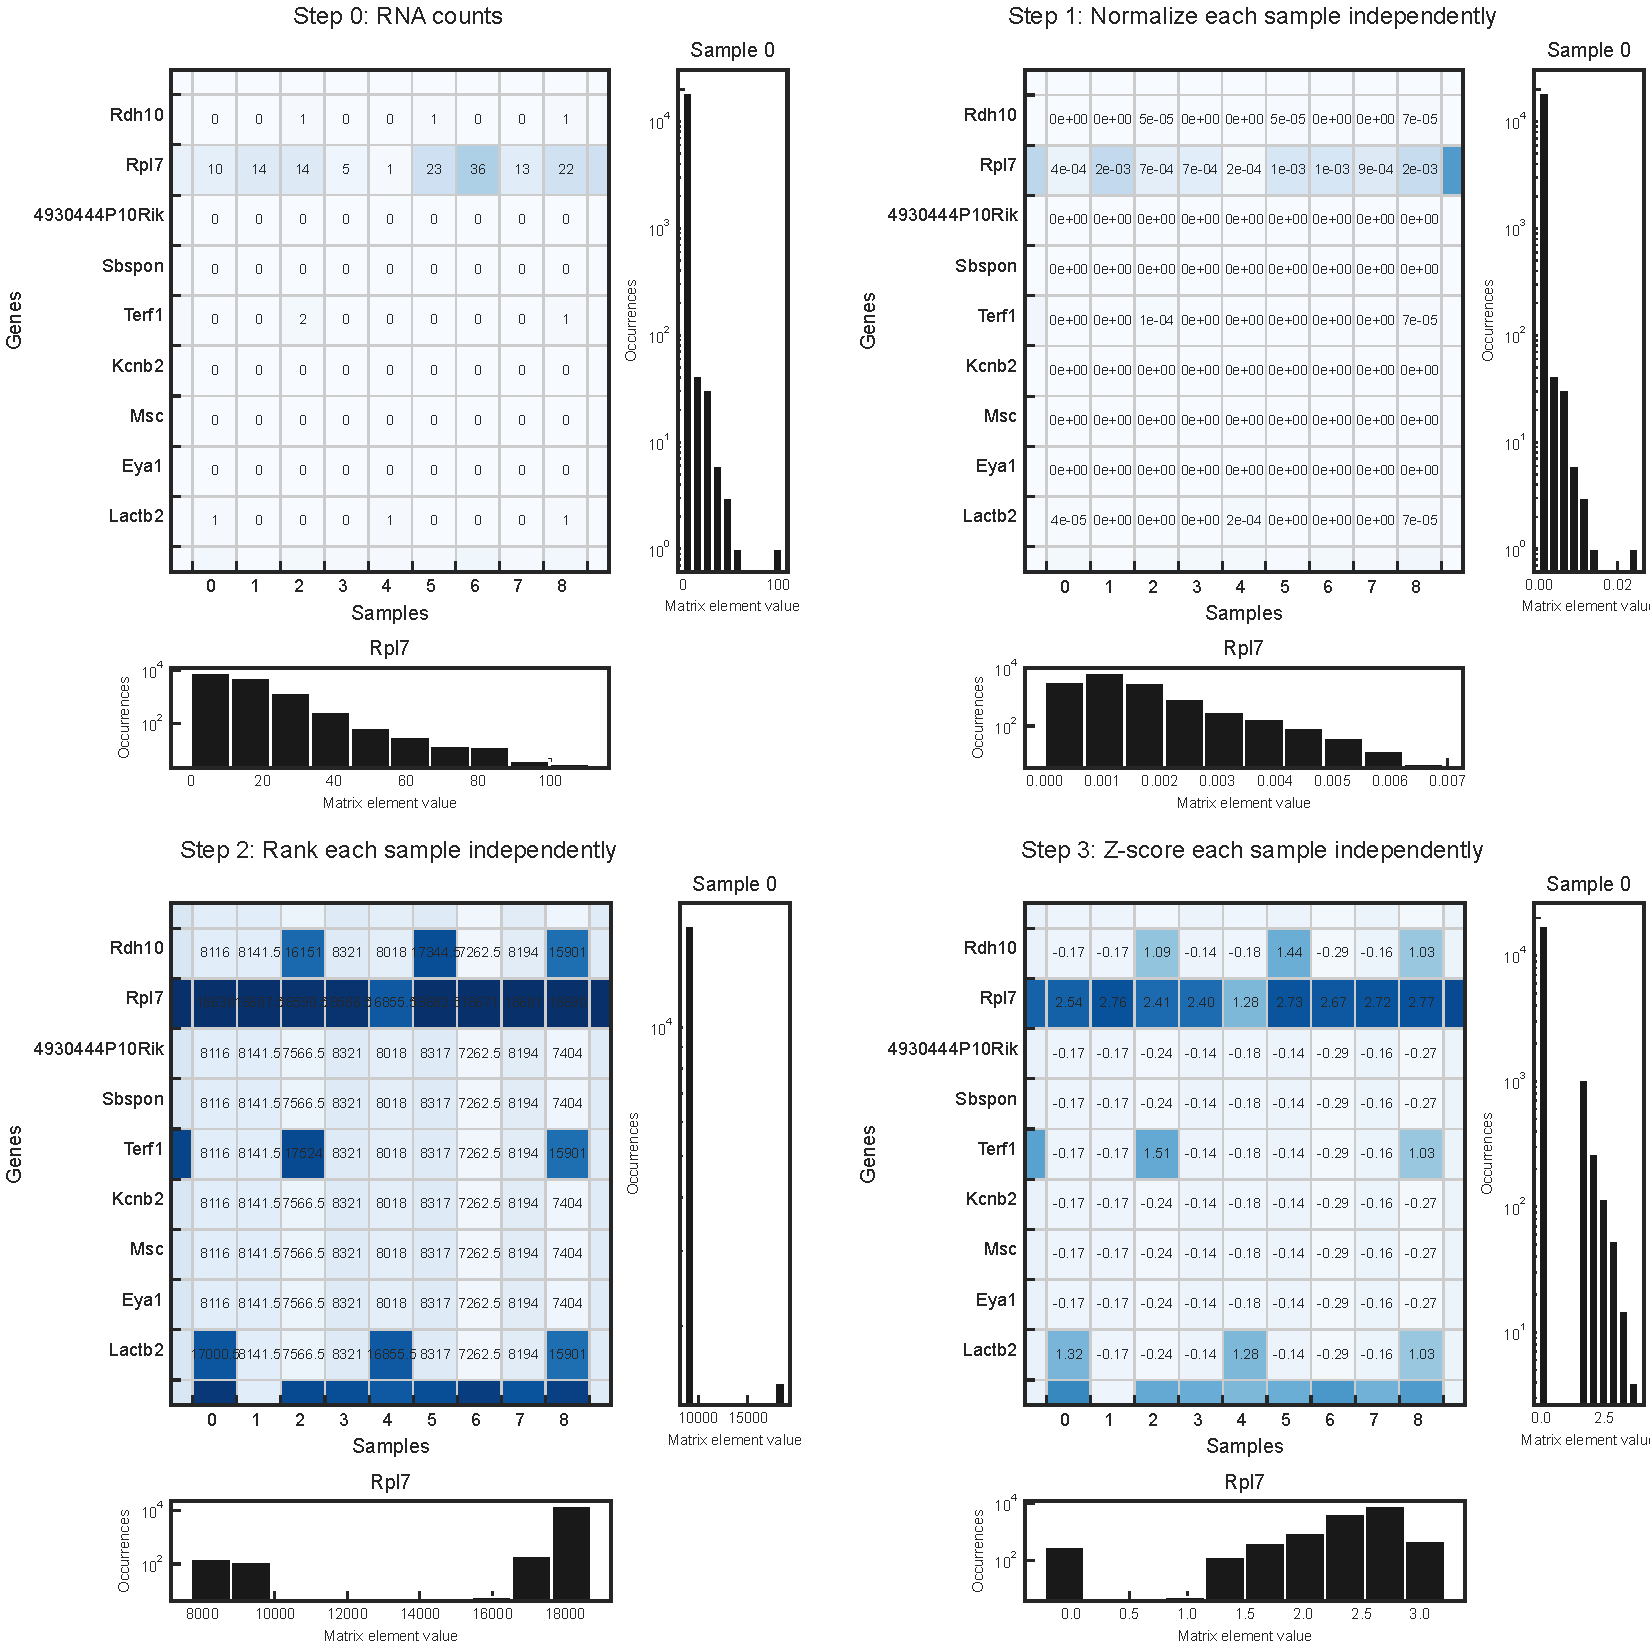
\includegraphics[scale=0.6]{figs/fig1a supplement.pdf}
	\caption{Data distributions at each pre-processing step}
	\label{FIG:supp1}
\end{figure}

\subsection{Analysis details \label{analysis}}
details on how ref. bases were constructed, specific things done for each dataset, etc.

describe accuracy scores + how only cells w. cell types represented in reference basis were analyzed. discuss how "unspecified" rate for unrepresented types (i.e. true negatives) was very high

Describe how MCA, TM, and subsets of data were used. number of cells taken. hill function discussion to explain how reference sample size affects scTOP score

hematopoiesis data: we excluded erythrocytes and (?) because only one marker gene was used to annotate the original data, which caused a lot of noise since using only one marker gene does not sufficiently isolate the red blood cell population

\subsection{Interpreting scores}
What scores are "high enough" or low, according to aggregate or individual

What a negative score means

How accuracies were calculated (what "unspecified" means)

\subsubsection{scTOP scores for irrelevant cell types}
Using same data as some of the figures in the main paper (ones that don't use the heatmap, since that already shows the irrelevant type scores are low), show that the false positive rate is very low

\subsection{Robustness of reference basis}
Show that the scores don't change significantly unless the reference basis is very bad. Show what happens when cell types are combined

\subsubsection{Cases where it doesn't work}\label{failure_cases}
All the cases where scTOP fails are expected; they are where the underlying assumption of "reference basis = attractor basins" is false

Stromal vs parenchyma (different levels of specialization)

When the reference basis is ill-defined (e.g. early in embryonic development, when cells aren't well-differentiated) (or when not enough cells are used for the archetypal gene expression profiles)

UMI vs non-UMI

\bibliography{export-data.bib}

\end{document}